\documentclass[%
 reprint,
%superscriptaddress,
%groupedaddress,
%unsortedaddress,
%runinaddress,
%frontmatterverbose, 
%preprint,
%showpacs,preprintnumbers,
%nofootinbib,
%nobibnotes,
%bibnotes,
 amsmath,amssymb,
 aps,
%pra,
%prb,
%rmp,
%prstab,
%prstper,
%floatfix,
]{revtex4-1}

\usepackage{graphicx}% Include figure files
\usepackage{dcolumn}% Align table columns on decimal point
\usepackage{bm}% bold math
%\usepackage{hyperref}% add hypertext capabilities
%\usepackage[mathlines]{lineno}% Enable numbering of text and display math
%\linenumbers\relax % Commence numbering lines

%\usepackage[showframe,%Uncomment any one of the following lines to test 
%%scale=0.7, marginratio={1:1, 2:3}, ignoreall,% default settings
%%text={7in,10in},centering,
%%margin=1.5in,
%%total={6.5in,8.75in}, top=1.2in, left=0.9in, includefoot,
%%height=10in,a5paper,hmargin={3cm,0.8in},
%]{geometry}

\usepackage{cmap} % Поиск в PDF
\usepackage[T2A]{fontenc} % Кодировка
\usepackage[utf8]{inputenc} % Кодировка исходного текста
\usepackage[english, russian]{babel} % Локализация и переносы
\frenchspacing % Более тонкая настройка пробелов 
\usepackage{multirow}
\usepackage[warn]{mathtext}
\usepackage{amssymb}
\usepackage{ dsfont }
\usepackage{ textcomp }
\usepackage{ mathrsfs }

% Переопределение англоязычного начертания каппа, фи и эпсилон, 
% а также знаков сравнения
\renewcommand{\epsilon}{\ensuremath{\varepsilon}}
\renewcommand{\phi}{\ensuremath{\varphi}} 
\renewcommand{\kappa}{\ensuremath{\varkappa}}
\renewcommand{\le}{\ensuremath{\leslant}}
\renewcommand{\leq}{\ensuremath{\leqslant}}
\renewcommand{\ge}{\ensuremath{\geslant}}
\renewcommand{\geq}{\ensuremath{\geqslant}}
\renewcommand{\emptyset}{\ensuremath{\varnothing}}

\usepackage{textcomp} 
\usepackage{indentfirst} % Красная строка
\usepackage{amsmath} % Текст в формулах
\usepackage{graphicx} % Графика
\DeclareGraphicsExtensions{.pdf,.png,.jpg}
\usepackage{pgfplots}
\pgfplotsset{compat=1.13}

%\usepackage{times}

\begin{document}

\title{Определение ширины запрещенной зоны полупроводника}
\thanks{11.1}

\author{Иван Едигарьев}
\affiliation{
 Московский Физико-Технический Институт\\
 Факультет Общей и Прикладной Физики, 526т\\
}
%\date{\today}

\begin{abstract}
Исследуется температурная зависимость проводимости типичного полупроводника - германия или кремния. Определяется ширина запрещенной зоны с помощью универсального цифрового вольтметра.

\end{abstract}

\pacs{Valid PACS appear here}

\maketitle

Измерим проводимость полупроводникового и медного образцов в зависимости от температуры.

Будем нагревать образцы от комнатной температуры до $100^{\circ}C$. Через каждые $5^{\circ}C$ будем измерять сопротивление полупроводникового и медного образцов, поочередно подключая их к прибору с помощью ключа K.

Используя соотношение
$$ \sigma = \frac{l}{RS},$$

построим график зависимости $\sigma(T)$ для обоих образцов. По наклону графика для медного образца определим температурный коэициент сопротивления меди.
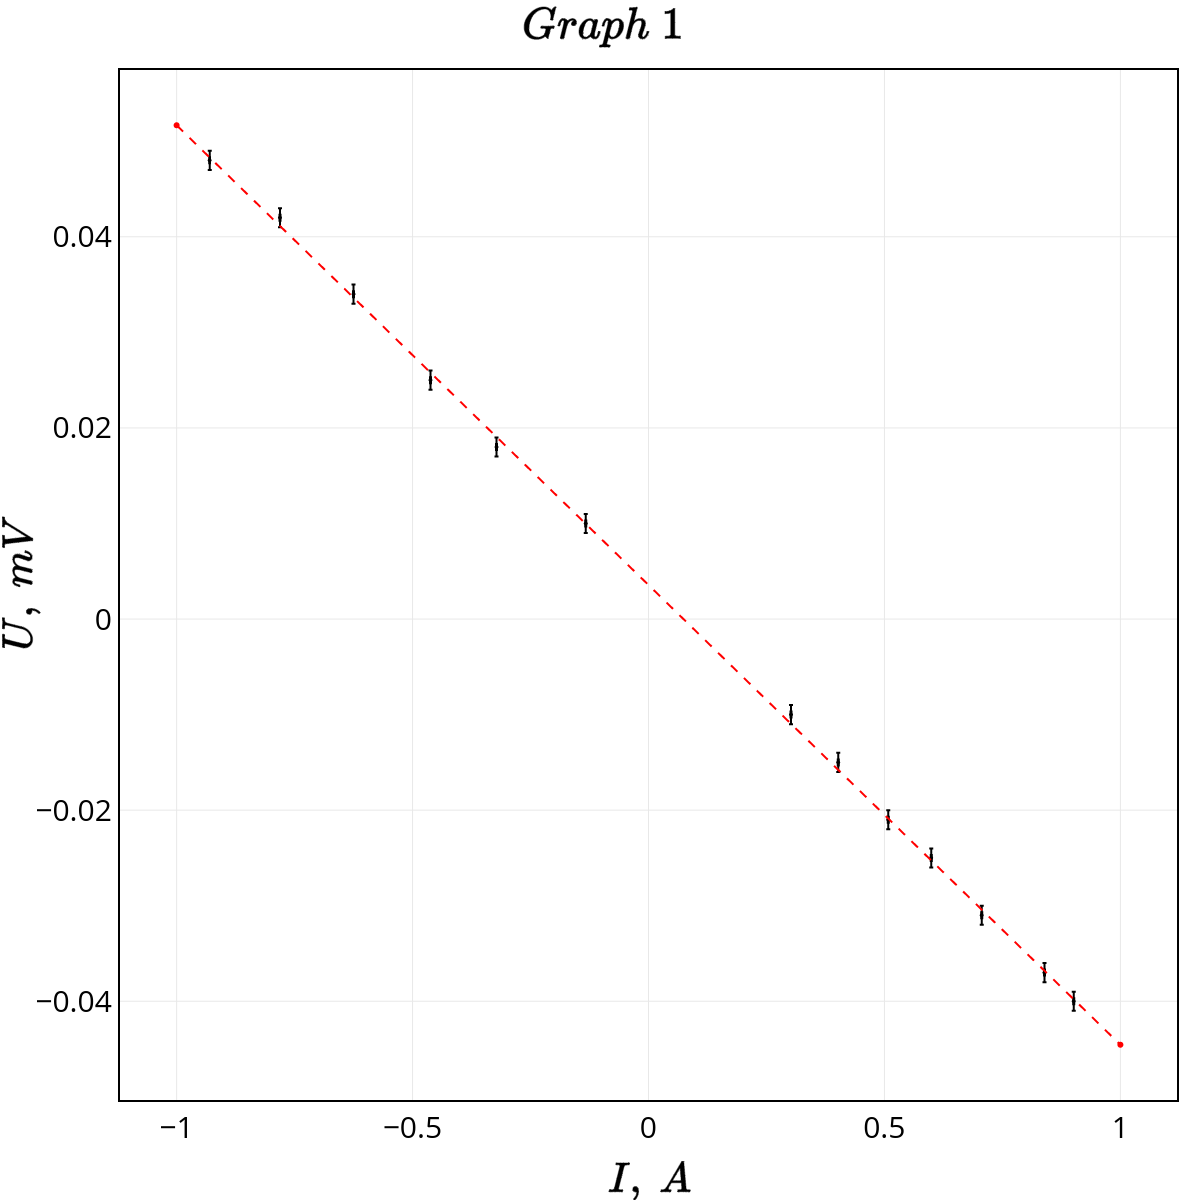
\includegraphics[scale=0.20]{my_plot1.png}
\begin{gather*}
\alpha_{cu} = \frac{1}{R}\frac{dR}{dT} = \sigma\frac{d}{dT}(\frac{1}{\sigma}) = - \frac{1}{\sigma}\frac{d\sigma}{dT} =  (3.5 \pm 0.2)~10^{-3}\cdot 1/K.
\end{gather*}
Построим график $\ln(\sigma) = f(1/T)$ для полупроводникового образца и по наклону его прямолинейной части (при более высоких температурах) определим ширину запрещенной зоны; выразим ее в электрон-вольтах.
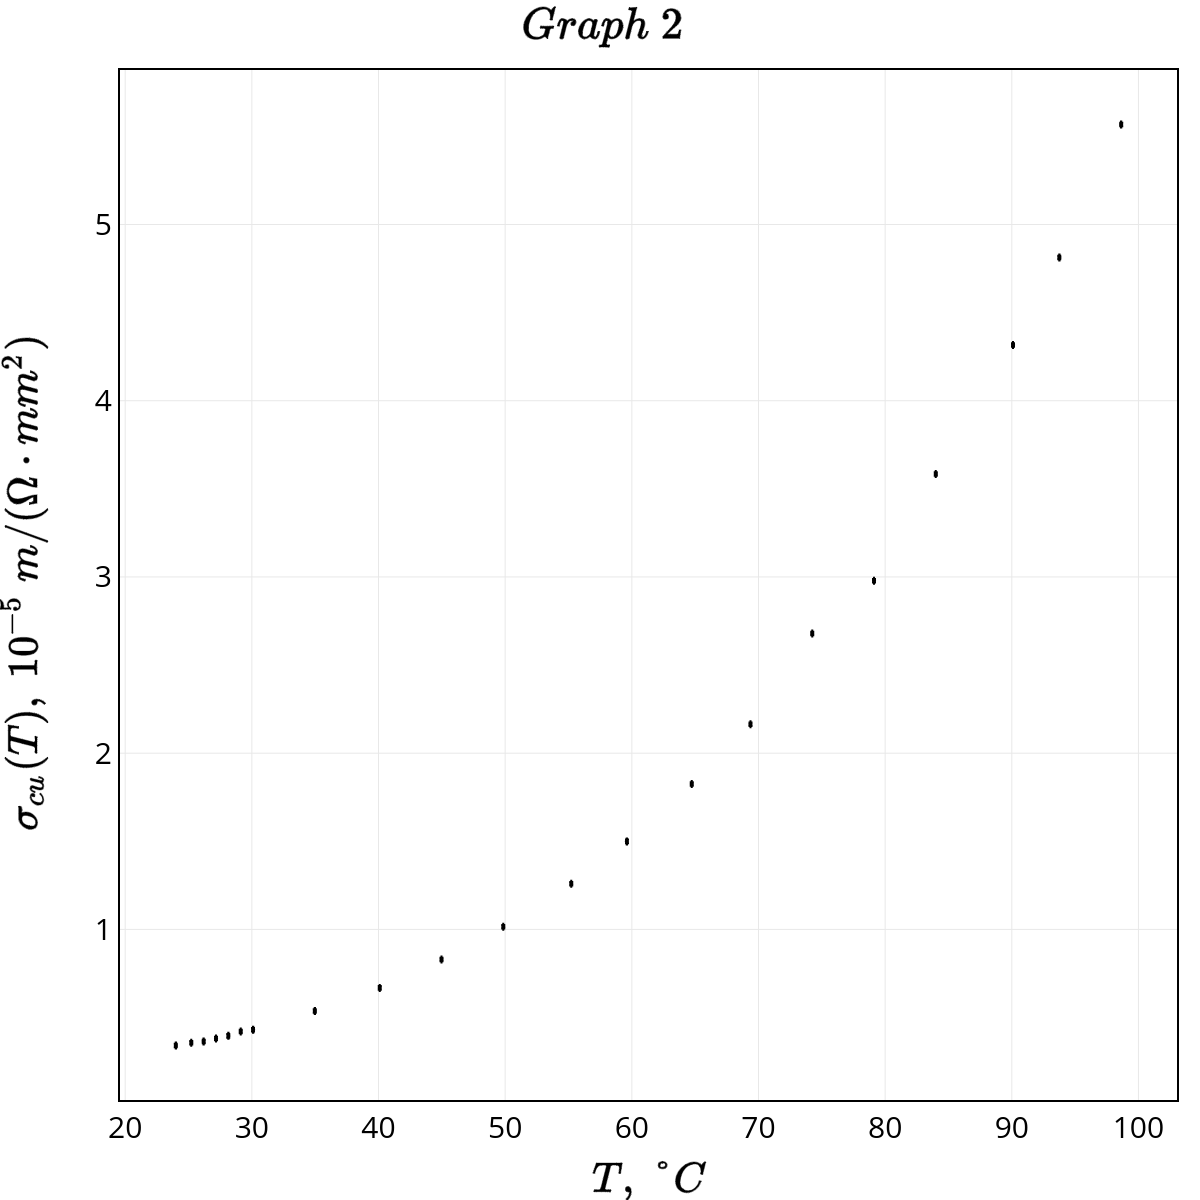
\includegraphics[scale=0.20]{my_plot2.png}
\begin{gather*}
\tg(\alpha) = \frac{\Delta}{2k_B} = 4.2 \cdot 10^{3}~K, \\
\Delta = (0.7 \pm 0.1)~eV.
\end{gather*}

По полученным значениям проводимости и ширины запрещенной зоны определим материал полупроводникового образца. В нашем случае можно сделать вывод о том, что в экспериментальной установке использовался германий.

Оценим достоверность полученных результатов в определении ширины запрещенной зоны исследуемого полупроводника и коэиффциента температурного сопротивления меди.

\begin{gather*}
\alpha_{cu} = 3.8\cdot10^{-3}~1/K, \\
\Delta_{table}^{Ge} = (0.67 \pm 0.1)~eV.
\end{gather*}

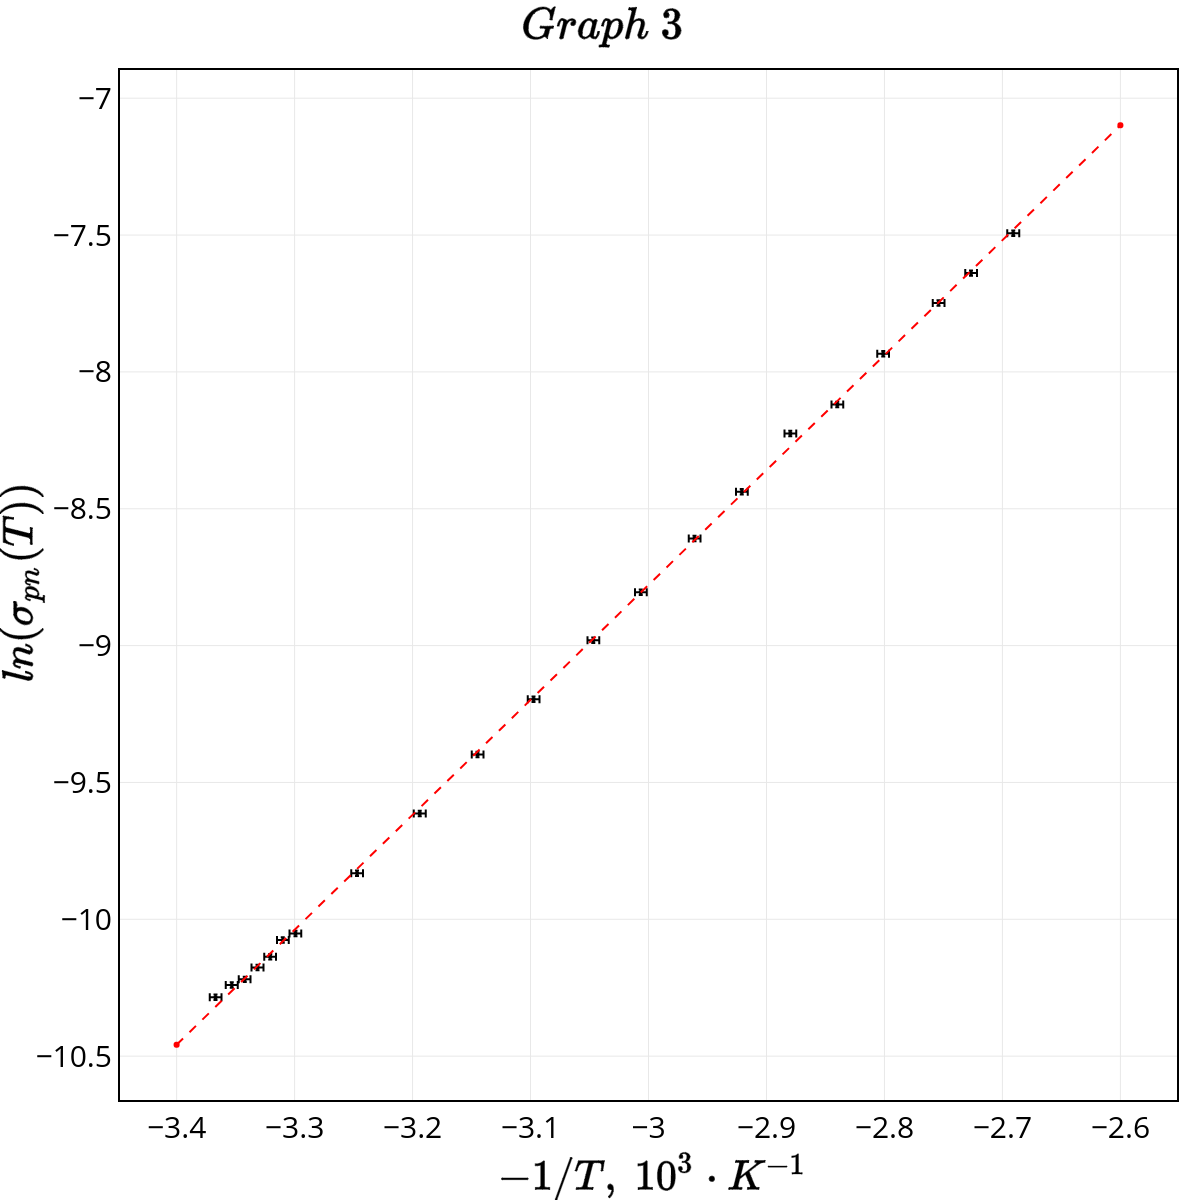
\includegraphics[scale=0.20]{my_plot3.png}

\end{document}